\chapter{Results}
\label{s:results}

\section{Euler}
One of the first tests for an ODE solver is whether it handles harmonic oscillations properly. The simple oscillations (shown in \ref{eq:osceq} with their analytical solutions) can be implemented as a matrix vector equation (\ref{eq:oscmatrix}), which represents two uncoupled oscillations of different frequencies. Besides the matrix of constants, the solver also requires initial values. For the first oscillation the initial position is non-zero, for the second oscillation the initial velocity is non-zero. 

\begin{align}
\label{eq:osceq} \nonumber
x_{0} '' &= - x_{0} \\
x_{2} '' &= -4 x_{2} \\ \nonumber
\\ \nonumber
\label{eq:osceqsol} \nonumber
x_{0}(t)  &= 50 \cos{(t)} \\ \nonumber
x_{2}(t)  &= 25 \sin{(2t)} \\ \nonumber
\end{align}


\begin{equation}
\label{eq:oscmatrix}
\vecb{x}' = \begin{bmatrix} 
0 & 1 & 0 & 0 \\
-1 & 0 & 0 & 0 \\
0 & 0 & 0 & 1 \\
0 & 0 & -4 & 0 \\
\end{bmatrix} \vecb{x} 
\hspace{20pt} \text{with} \hspace{20pt} 
\vecb{x}(t = 0) =\begin{bmatrix} 50 \\ 0 \\ 0 \\ 50 \end{bmatrix} 
\end{equation}


\begin{figure}[h]
	\centering
	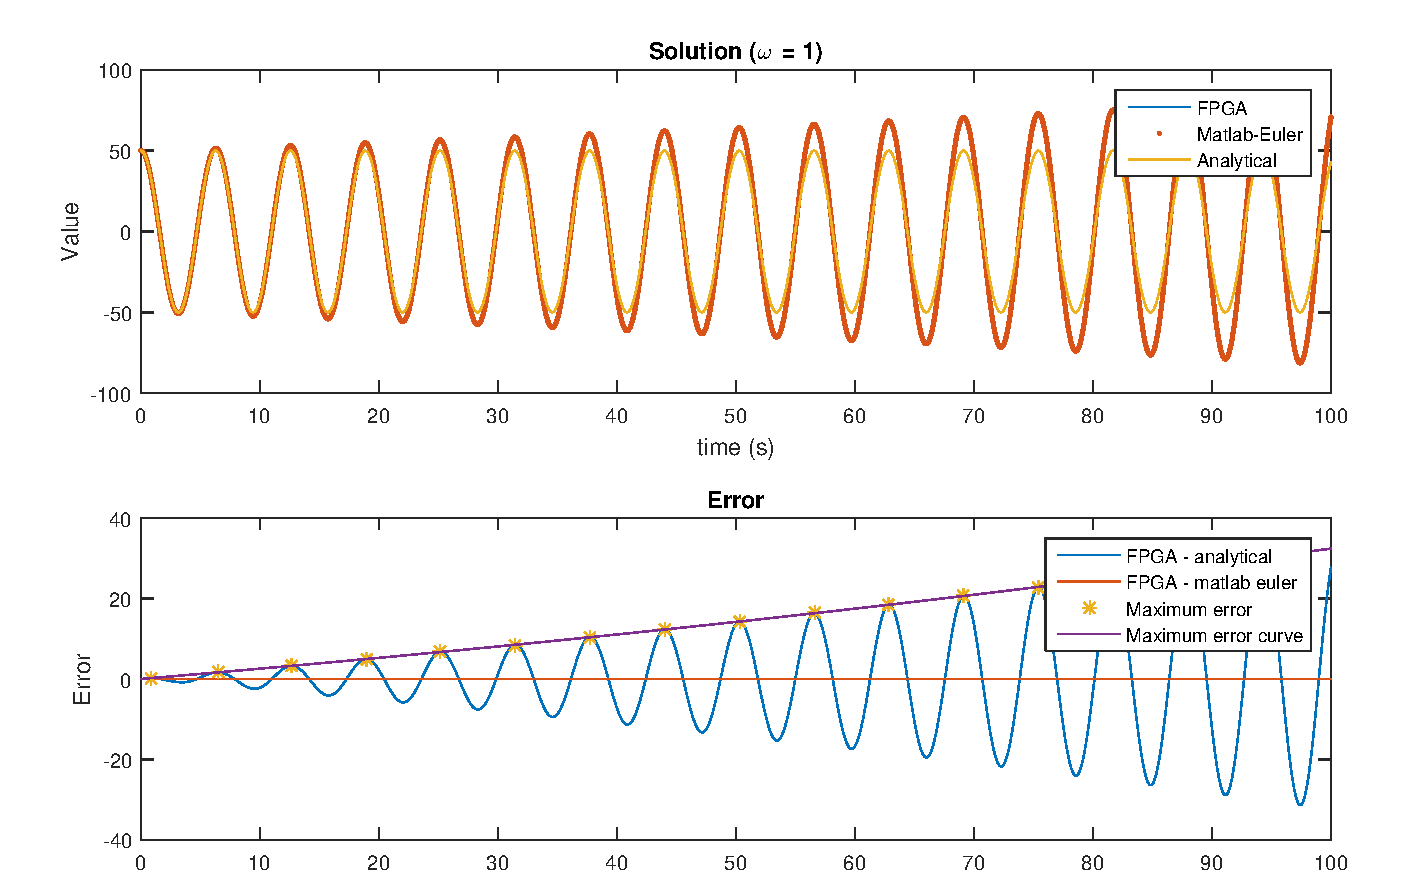
\includegraphics[width=\textwidth]{euler_o1_ts=0,01_os=1}
	\caption{Simple oscillation using Euler's method (h = 0.01)}
	\label{f:euler_o1_ts=0,01_os=1}
\end{figure}

\subsection{First oscillation - initial position}
The plots belonging to the first oscillation (\ref{f:euler_o1_ts=0,01_os=1}) depict three variations on solving the system. Firstly, it contains the solution generated by the FPGA. Secondly, it contains the result of the exact same combination of equation and solver, but implemented in \matlab{}. The only difference between the FPGA and \matlab{} implementation is the number representation. Therefore, if the FPGA solution starts to diverge from the \matlab{} solution the reason has to be the reduced accuracy of the 32-bit fixed point representation used in the FPGA. Internally, \matlab{} uses a (64-bit) double precision floating format \cite{MatlabFloat}, which is guaranteeing a precision of ~15 significant figures for almost all magnitudes supported by the IEEE 754 double precision floating point standard. Lastly, the plot contains the analytical solution of the problem.

The plot shows that the FPGA exhibits the expected behaviour of solving a simple oscillation with Euler's method. Due to the relatively large step size (h = 0.01) the approximation quickly diverges from the analytical solution. The curvature of the solution is always opposite in sign to the solution itself ($x'' = -x$), which results in a self-amplifying effect in the magnitude of the error: an exponential error growth. This was expected, as the exponential dependency was already derived by \cite{DE} in equation \ref{eq:euler_error}. However, this does show that Euler's method is a particularly bad integration scheme for a simple oscillation. It is possible to use \matlab{}s Curve Fitting Tool to fit the equation of the theoretical maximum error of Euler's method to the points of maximum error. After combining some constants, \ref{eq:euler_error} becomes equal to \ref{eq:euler_error_combined}. For $a = 49.75$ and $b = 0.00502$ this equation achieves a fit of $R^{2} = 1$, which is a perfect fit. The error plot and the curve fit of the maximum errors are shown in \ref{f:euler_o1_ts=0,01_os=1}.

\begin{equation}
\label{eq:euler_error_combined}
\text{error}_{\text{euler}}(t) = a (e^{b t} - 1)
\end{equation}

Lastly, the FPGA solution the solution of Euler's method implemented in \matlab{} shows that the error due to the fixed point number representation is clearly insignificant when compared to the intrinsic error in Euler's method: the maximum absolute difference between the two solutions is less than 6\e{-5}.

\subsubsection{Decreasing the time step - improving accuracy?}
The expectation based on \cite{DE} and equation \ref{eq:euler_error} is that the maximum error is indeed proportional to the time step, meaning that a hundred fold decrease of the time step also decreases the error by a factor 100. The maximum error at $t \approx 100$ for $h = 0.01$ was $\approx 30$, whereas the maximum error for $h = 0.0001$ is $\approx 0.2$, which is an improvement of $150 \times$, 50\% more than expected. However, even though the error relative to the analytical solution has decreased, the divergence from the \matlab{} implementation of Euler's algorithm has increased to 8\e{-4}, a factor of 13.

As the time step gets decreased even more, eventually the improvement of having a shorter time step loses out to the reduction the accuracy in the computation. This can be seen very clearly in \ref{f:euler_o1_ts=0,0000001_os=1000}. Featuring a time step of h = 1 \e{-7}, which is approaching the smallest representable value at $2^{-24}$. In this case the \matlab{} implementation is still following the analytical solution with little whereas the solution generated by the FPGA begins to diverge noticeably.

\begin{figure}[h]
	\centering
	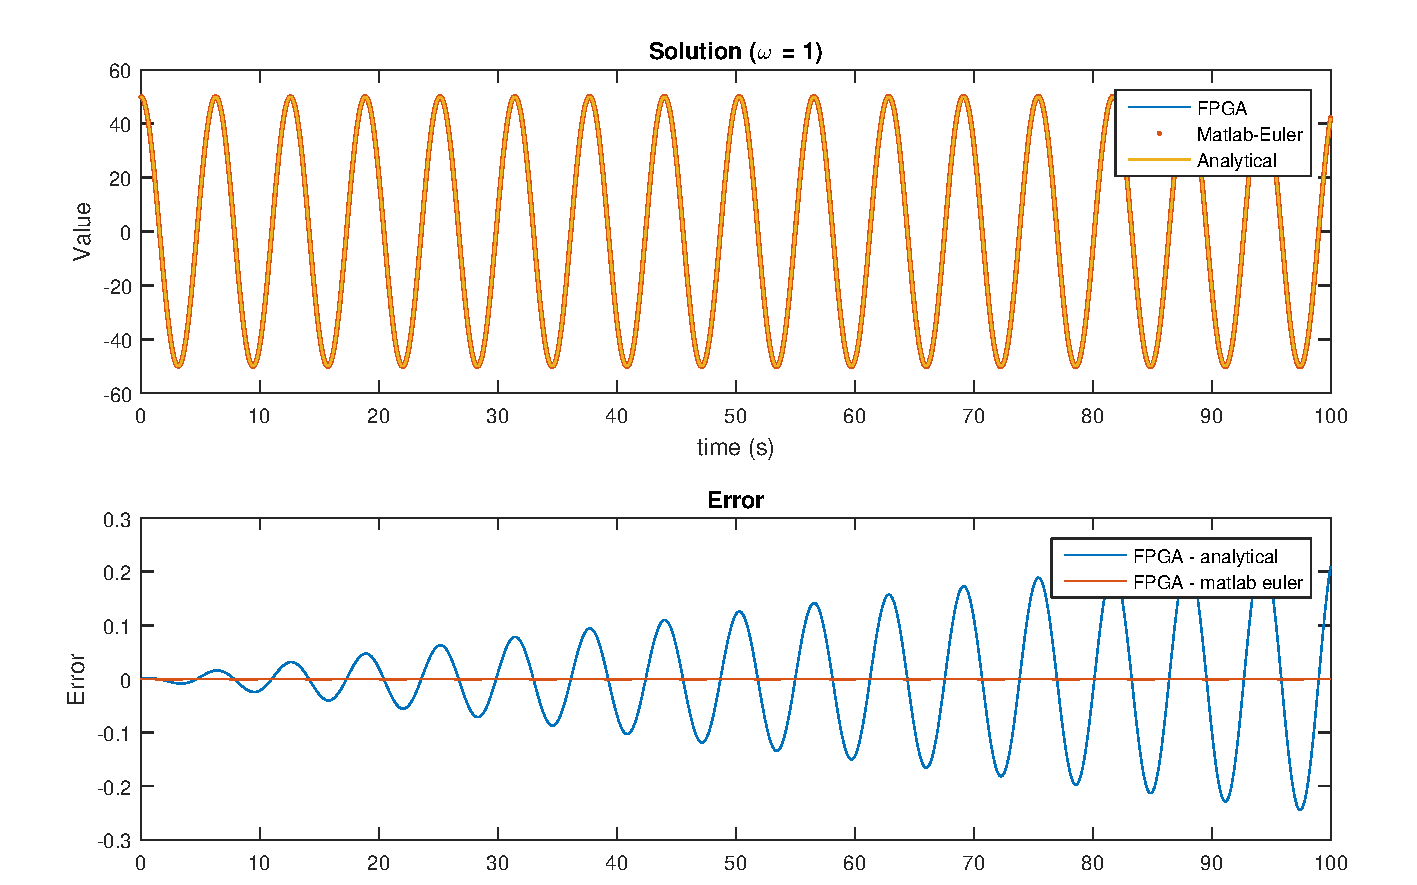
\includegraphics[width=\textwidth]{euler_o1_ts=0,0001_os=100}
	\caption{Simple oscillation using Euler's method with a lower time step (h = 1 \e{-4})}
	\label{f:euler_o1_ts=0,0001_os=100}
\end{figure}

\begin{figure}[h]
	\centering
	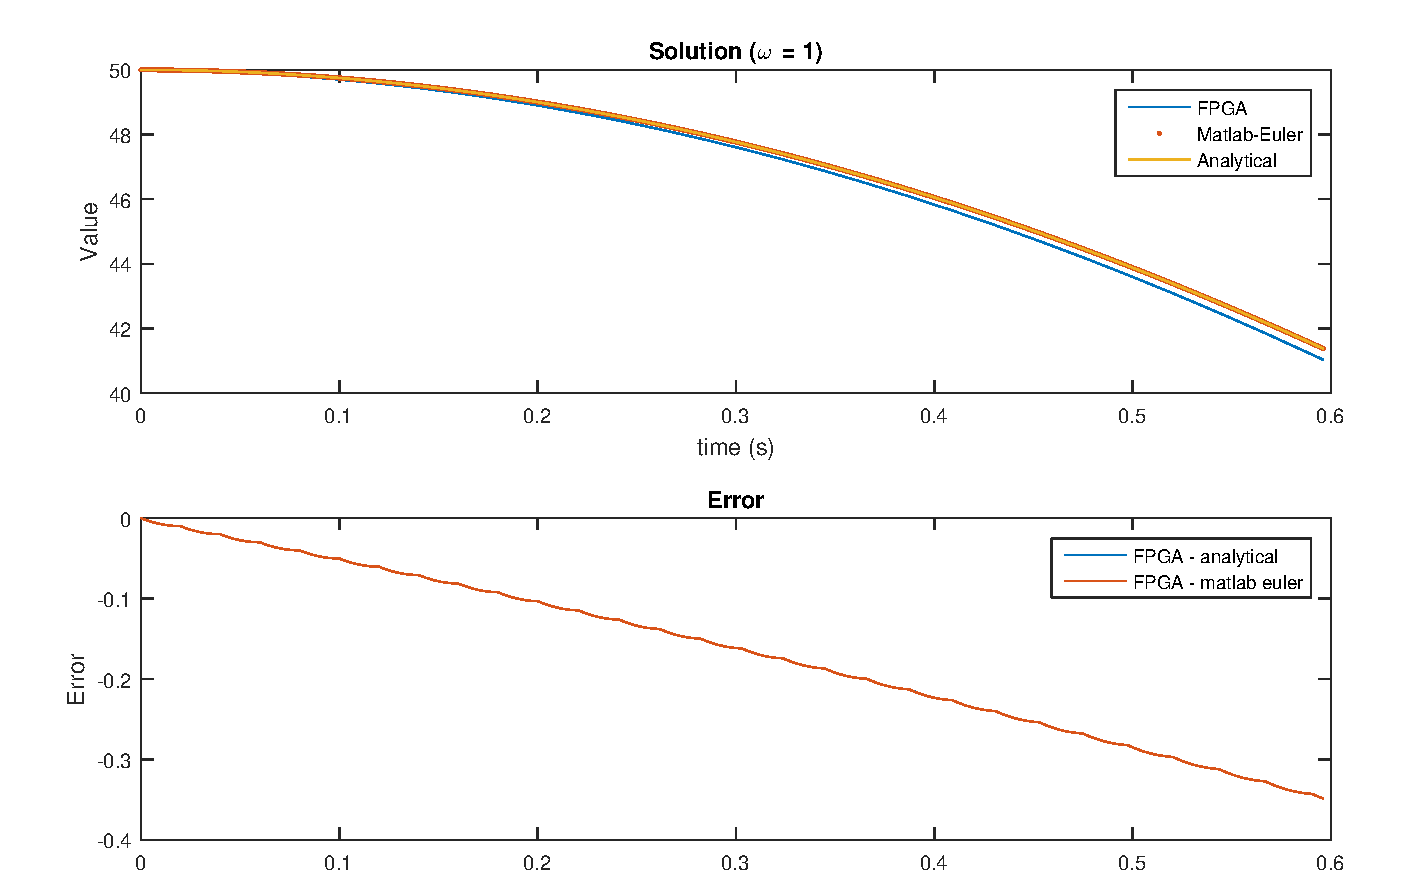
\includegraphics[width=\textwidth]{euler_o1_ts=0,0000001_os=1000}
	\caption{Approaching breakdown due to the fixed point number representation (h = 1 \e{-7})}
	\label{f:euler_o1_ts=0,0000001_os=1000}
\end{figure}

\subsection{Second oscillation - initial velocity}
Similarly to the previous scenario, the error increases exponentially over time and an decrease in time step is approximately proportional to the decrease in error (figure \ref{f:euler_o2_ts=0,001_os=100} and \ref{f:euler_o2_ts=0,00001_os=1000}). However, there is an important difference between the two oscillations: the frequency of oscillation is higher. This has as result that the time step of $h = 0.01$ which worked fine for the oscillation with $\omega = 1$ does not work properly any more: it results in figure \ref{f:euler_o2_ts=0,01_os=1}. This figure shows two interesting phenomena. Firstly, even though \matlab{}s Euler's method does diverge from the analytical solution, it only diverges in magnitude: it stays in phase. However, when looking at the FPGA solution you notice that it diverges from the other two, not only in magnitude but also in phase. The discrepancy in phase between \matlab{} and FPGA indicates that the number representation is the culprit of the shift. 

An attempt to fix this problem was made by changing the relevant part of the matrix from $\left[ \begin{smallmatrix} 0 & 1\\ -4 & 0 \end{smallmatrix} \right]$ to $\left[ \begin{smallmatrix} 0 & 2\\ -2 & 0 \end{smallmatrix} \right]$, which should have the result that the numbers remain smaller internally as the multiplication by 4 is distributed over two multiplications by 2 in separate vector dot products. Even though both matrices result in the same second order equation ($x'' = -4x$) and the eigenvalues are the same, the eigenvalues are different which results in different behaviour for the two matrices.  

\begin{figure}[h]
	\centering
	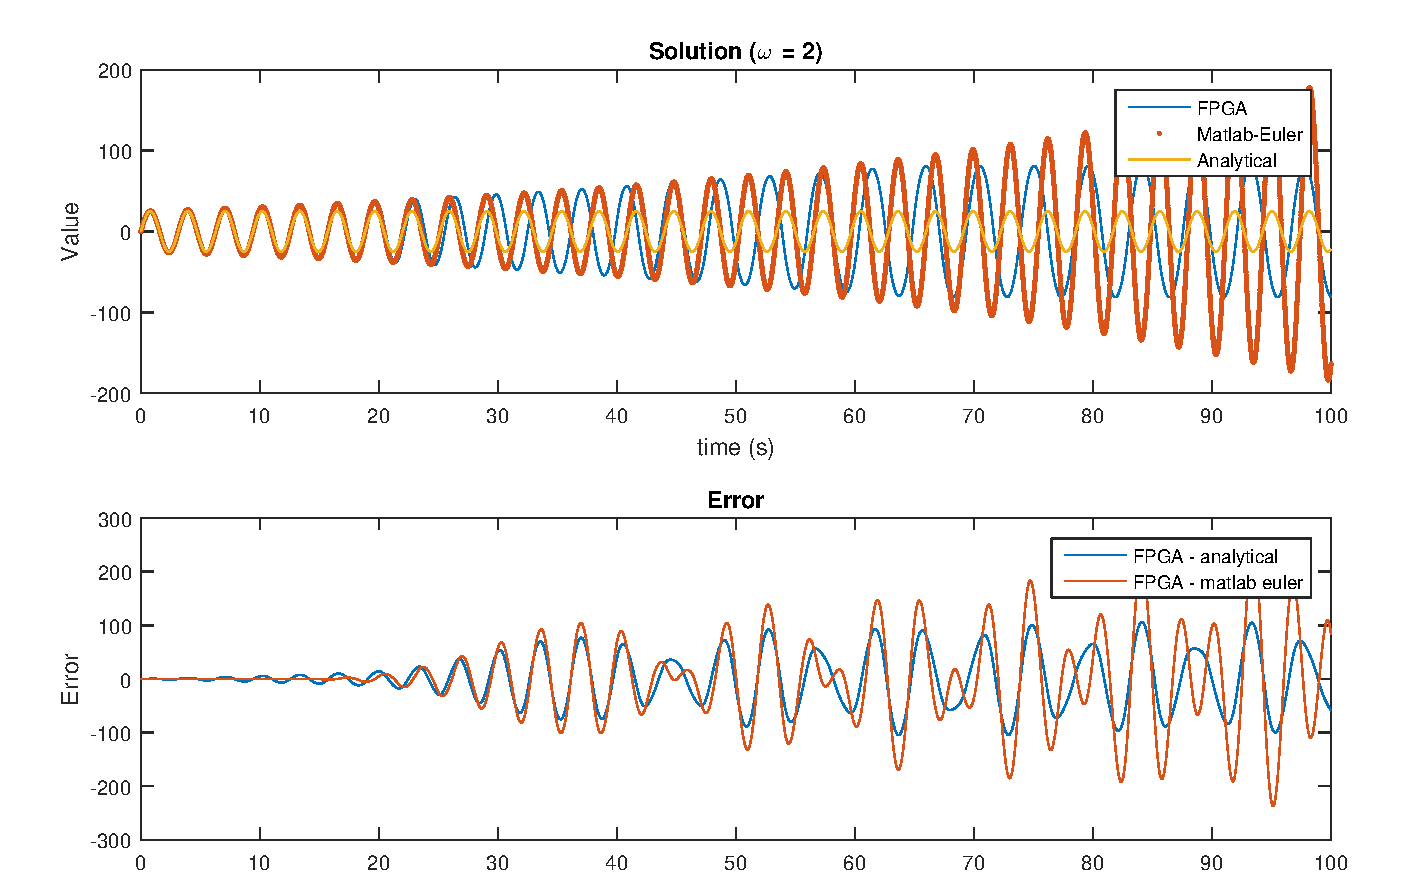
\includegraphics[width=\textwidth]{euler_o2_ts=0,01_os=1}
	\caption{Frequency shifting due to an insufficiently small time step (h = 0.01)}
	\label{f:euler_o2_ts=0,01_os=1}
\end{figure}

\begin{figure}[p]
	\centering
	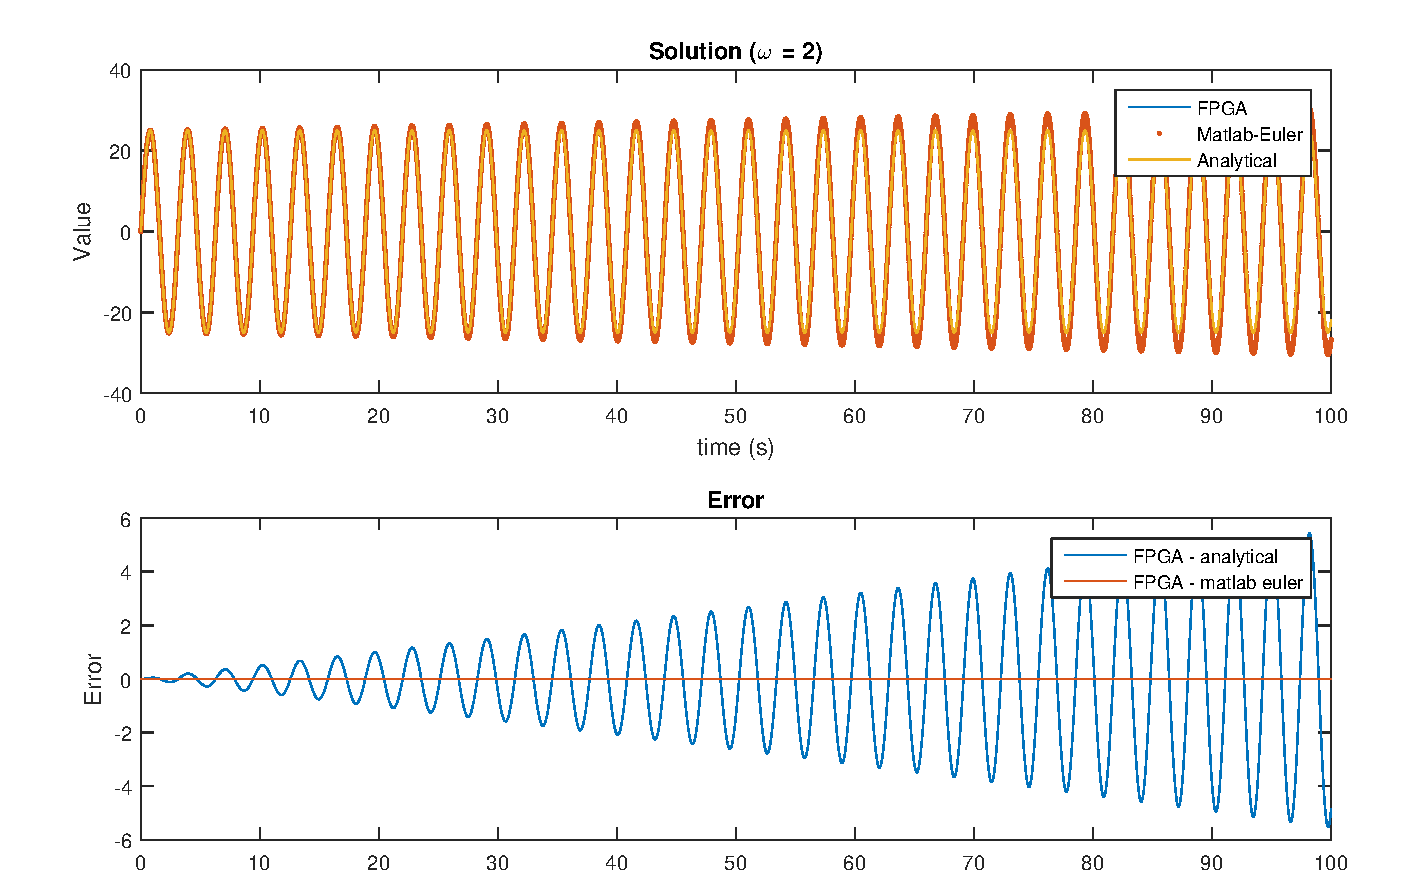
\includegraphics[width=0.95\textwidth]{euler_o2_ts=0,001_os=100}
	\caption{Relatively large time steps result in large errors in the long run (h=0.001)}
	\label{f:euler_o2_ts=0,001_os=100}
\end{figure}

\begin{figure}[p]
	\centering
	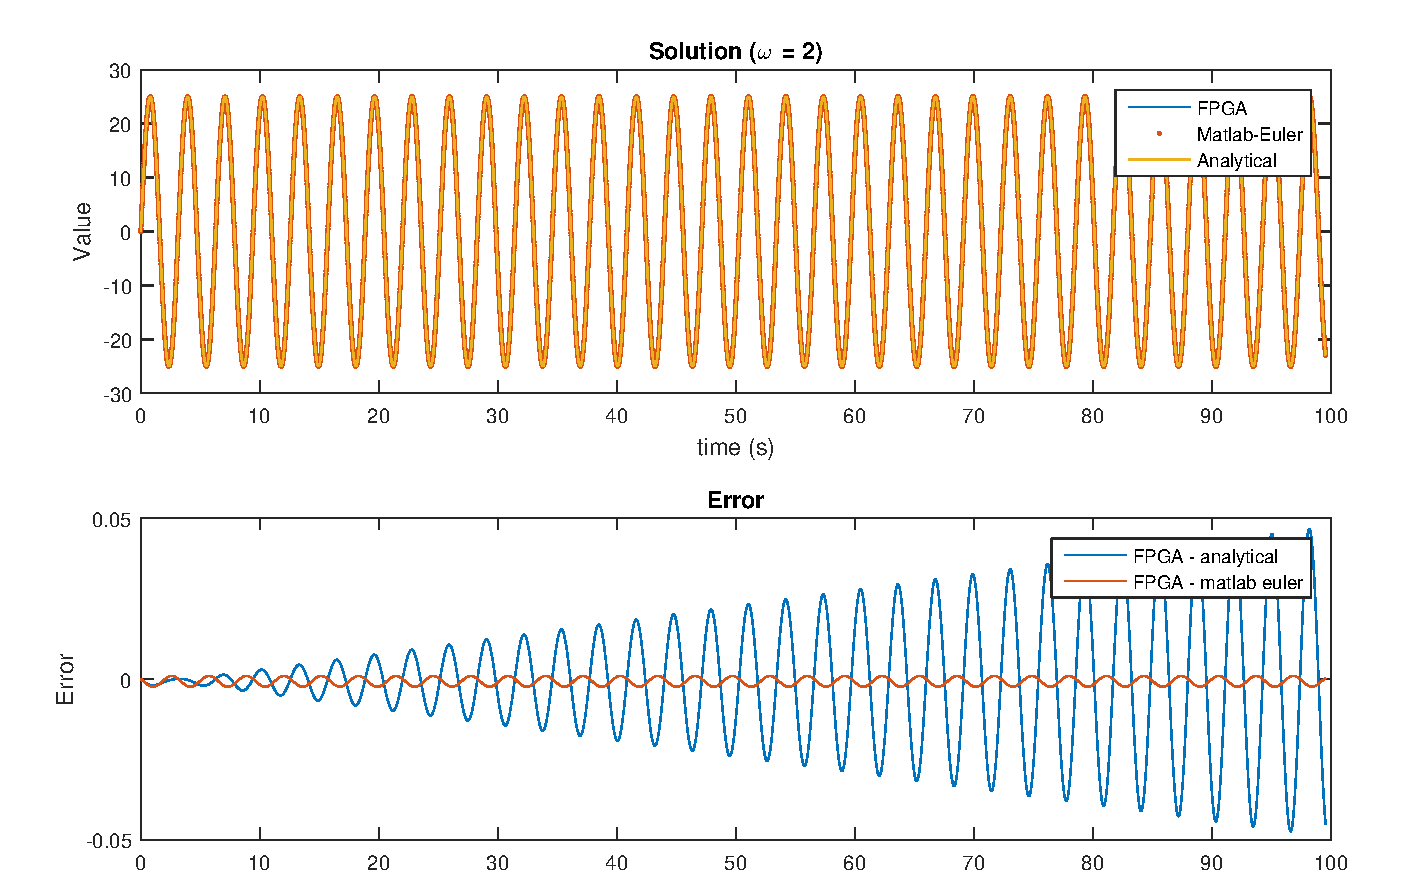
\includegraphics[width=0.95\textwidth]{euler_o2_ts=0,00001_os=1000}
	\caption{But a decrease in time step goes a long way in reducing the error. Note that the error due to the fixed point number representation starts to become significant again, in contrast to figure \ref{f:euler_o2_ts=0,001_os=100} (h = 1 \e{-5})}
	\label{f:euler_o2_ts=0,00001_os=1000}
\end{figure}

\section{Runge-Kutta (second order)}
The testing of the RK2 method uses a different matrix (equation \ref{eq:rk2matrix}) in order to verify the systems capability to correctly solve a system of 4, coupled, first order equations. The matrix has been generated randomly in \matlab{} under the constraint that all eigenvalues are negative. The reason as to why this property is necessary is, again, based on the fixed point number representation. Whenever one of the values (which could even occur internally as part of a vector dot product, invisible to interface) exceeds the allowed range, the result becomes invalid. If all elements in the vector described by the ODE tend towards zero, this problem is less likely to occur (but it might still happen whenever the initial conditions that have been chosen are too large). Furthermore, the added computational steps of RK2 compared to Euler's method have the effect that the time step becomes less important - for the entire range of possible time step values the results and errors are approximately the same (shown in figure \ref{f:rk2_ts=0,01_os=1} and \ref{f:rk2_ts=0,0000005_os=1000}). Lastly, in contrast to the FPGA solution, \matlab{} RK2 and ODE45 do remain close together which, once again, points in the direction of problems stemming from the fixed point numbers.

\begin{equation}
\label{eq:rk2matrix}
\vecb{x}' = \begin{bmatrix} 
2 & 3 & 2 & 0 \\
-5 & -5 & -3 & 1 \\
3 & -1 & -2 & -3 \\
4 & 2 & 2 & -3 \\
\end{bmatrix} \vecb{x} 
\hspace{20pt} \text{with} \hspace{20pt} 
\vecb{x}(t = 0) =\begin{bmatrix} 7 \\ 5 \\ 7 \\ 5 \end{bmatrix} 
\end{equation}

\begin{figure}[p]
	\centering
	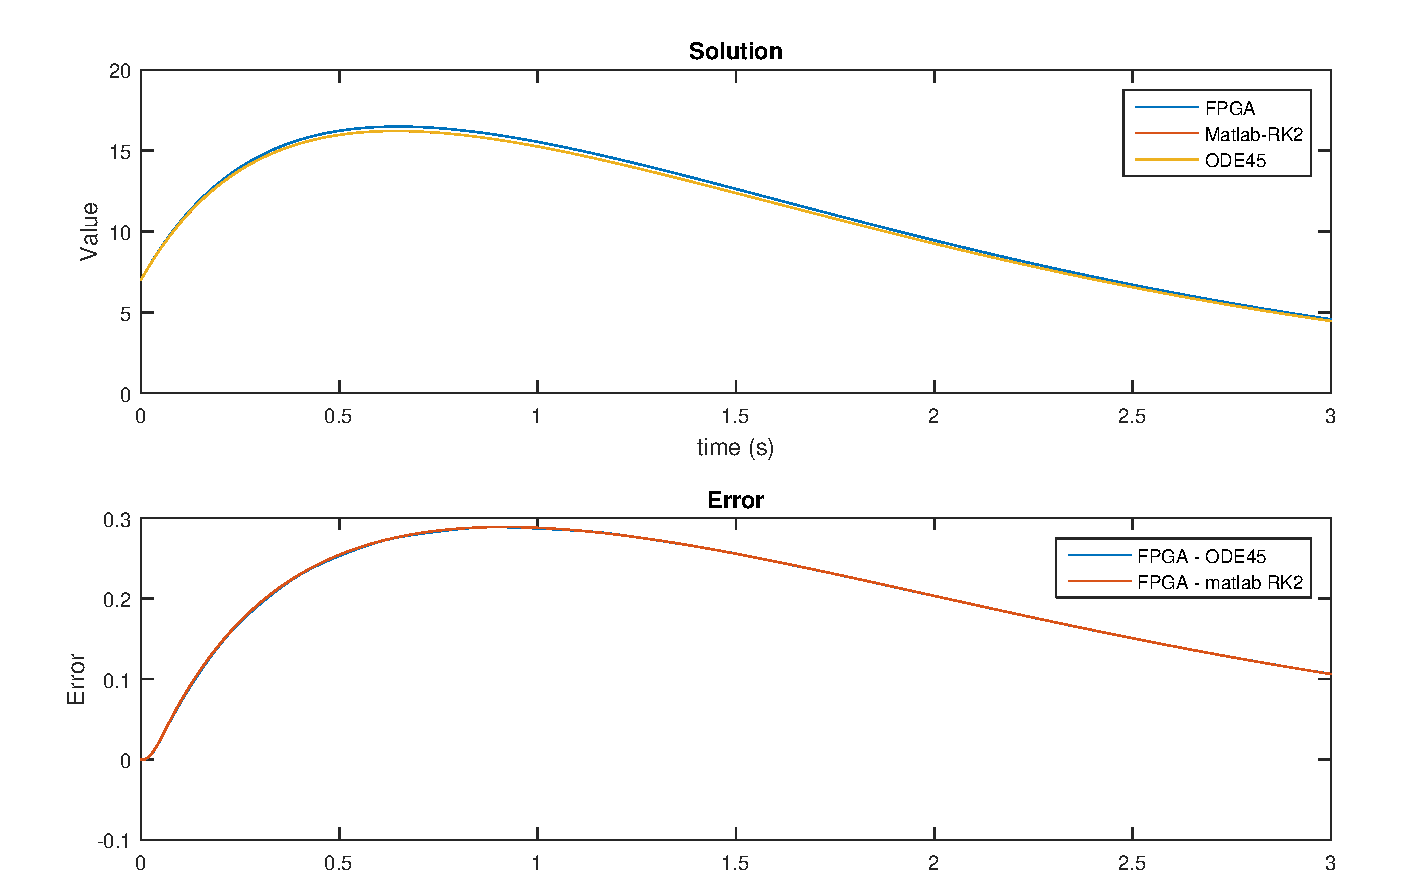
\includegraphics[width=0.95\textwidth]{rk2_ts=0,01_os=1}
	\caption{The largest possible time step has a maximum error of approximately 0.3, for both the comparison with the solution of ODE45 and \matlab{}s RK2 (h=0.01).}
	\label{f:rk2_ts=0,01_os=1}
\end{figure}

\begin{figure}[p]
	\centering
	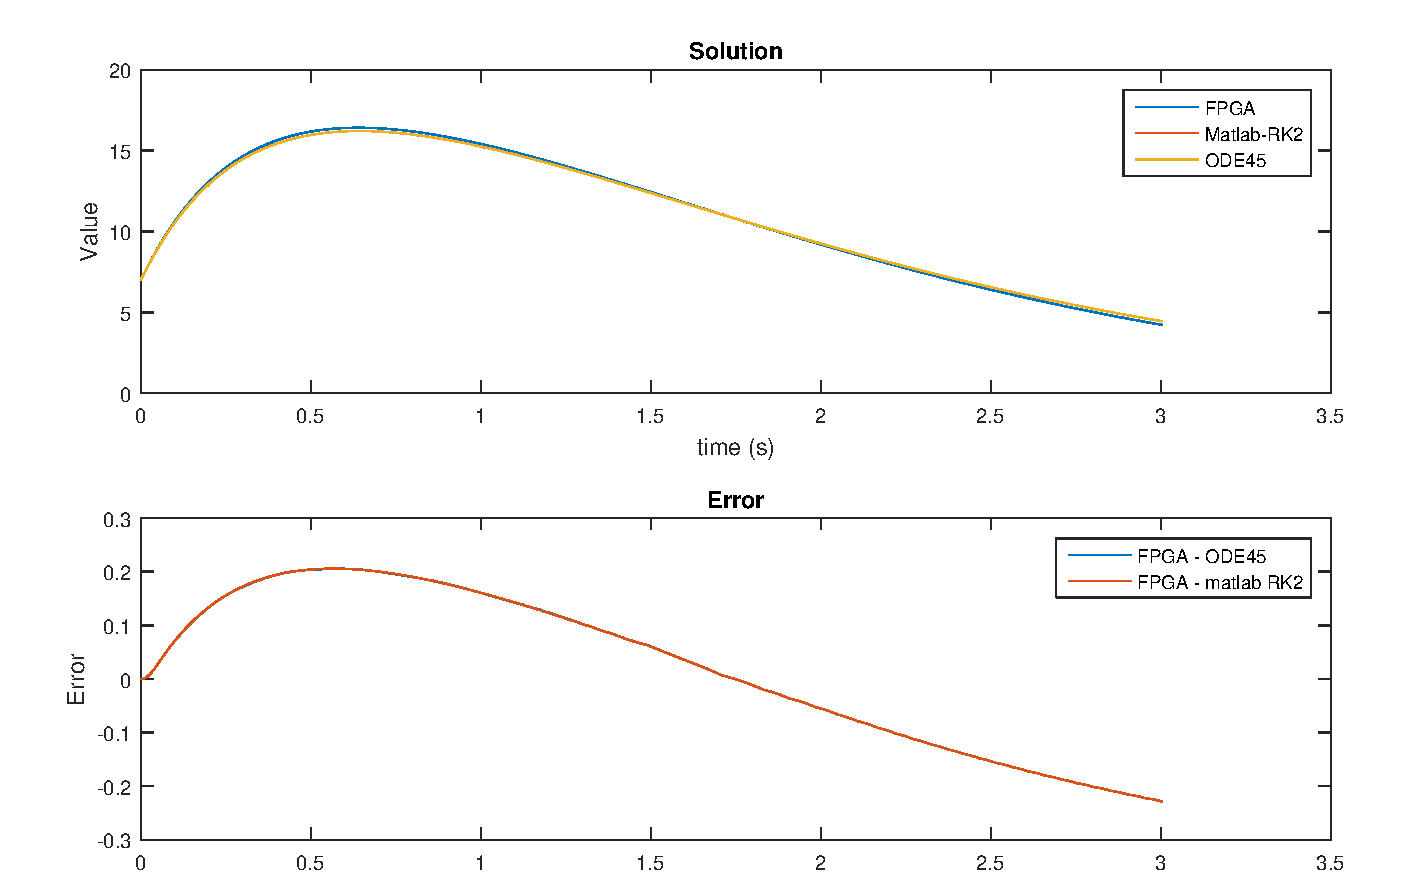
\includegraphics[width=0.95\textwidth]{rk2_ts=0,0000005_os=1000}
	\caption{Considering the other end of the spectrum regarding variety in time steps, the results do not differ significantly enough for the additional amount of work that has to be put in, a factor 20000 (h=5\e{-7}).}
	\label{f:rk2_ts=0,0000005_os=1000}
\end{figure}

\section{Runge-Kutta (fourth order)}
The RK4 integration scheme \footnote{Which took almost 22 hours or 78894 seconds to synthesize.} introduces even more computational steps, which leads to a faster overflow of the internal numbers. This means that at least one of the derivatives overflows almost immediately, which results in plots as shown in figure \ref{f:rk4_ts=0,00001_os=100}.


\begin{figure}[h]
	\centering
	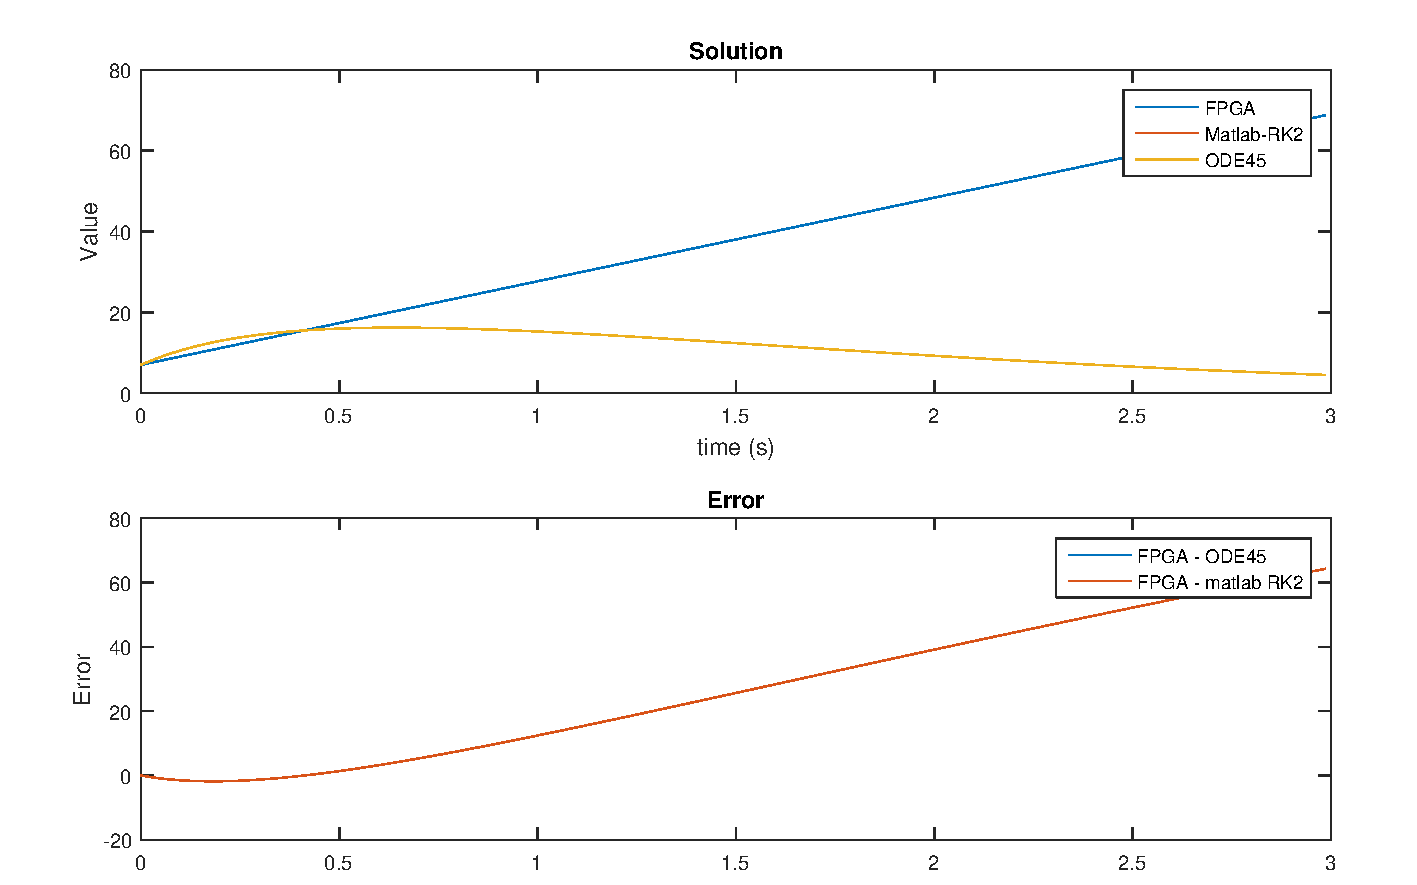
\includegraphics[width=\textwidth]{rk4_ts=0,00001_os=100}
	\caption{For every value of the time step the numbers overflow, causing derivatives to get stuck, resulting in straight lines instead of solutions to ODEs (h=1\e{-5}).}
	\label{f:rk4_ts=0,00001_os=100}
\end{figure}

\section{Euler revisited}
So far it appears that accuracy is inversely proportional to the complexity of the integration scheme, which leads to the question: What accuracy would Euler's method attain for equation \ref{eq:rk2matrix}? Indeed, as shown in figure \ref{f:euler_rv_ts=0,0001_os=10}, Euler's method only reaches maximum errors which are 2 orders of magnitude lower than the best values of the time step for RK2 and of course performs better than RK4 in this scenario. 

\section{Performance - add to conditions to appendix maybe?\textbf{}}
Performance is one of the main reasons why people use FPGAs over implementations in software and therefore one would expect that a properly written FPGA solution outperforms a CPU. The FPGA used for testing in this thesis is a Cyclone V, which, according to \cite{AlteraFPGA}, is meant for "your low-power, cost-sensitive design needs, enabling you to get to market faster". Furthermore, Altera offers two other FPGA families: Stratix and Arria, which both have mentions of delivering high or optimal performance. 

The FPGA runs at a clock speed of 50 MHz and it is capable of executing a single iteration of Euler's method per clock cycle. In theory this would mean that the FPGA is capable of 50\e{6} iterations per second. However, there is still quite some overhead stemming from the system handling the data input and output, which has to wait for the HPS to supply or request the proper information before the FPGA can move on with the computations.

\begin{table}
	\caption{Performance benchmarks: Euler's method}
	\label{t:perfomance}
	\begin{tabular}{l l l l l l}
		Device 	& Iterations& time (s)	& Output every	& Loop bound	& Iterations per second (\e{6}) \\  
		FPGA 	& 1\e{8} 	& 6,53		& 1.000			& 75			& 15,3 	\\
		FPGA 	& 1\e{8} 	& 4,61		& 10.000		& 750			& 21.7 	\\
		FPGA 	& 1\e{8} 	& 4,50		& 100.000		& 7.500			& 22,2 	\\
		FPGA 	& 1\e{8} 	& 4,36		& 100.000.000	& 7.500.000		& 22,9 	\\
		FPGA 	& 1\e{7} 	& 0,77		& 10.000.000	& 750.000		& 13,0 	\\
		FPGA 	& 1\e{6} 	& 0,42		& 1.000.000		& 75.000		& 2,3 	\\
		FPGA 	& 1\e{8} 	& 0,39		& 100.000		& 7.500			& 0,3 	\\
		CPU (i7)& 5\e{7} 	& 20,25		& 50.000.000	& -				& 2,5 	\\
		MATLAB 	& 1\e{7} 	& 303,83	& 10.000.000	& -				& 0,03	\\
	\end{tabular}
\end{table}

\begin{figure}[h!]
	\centering
	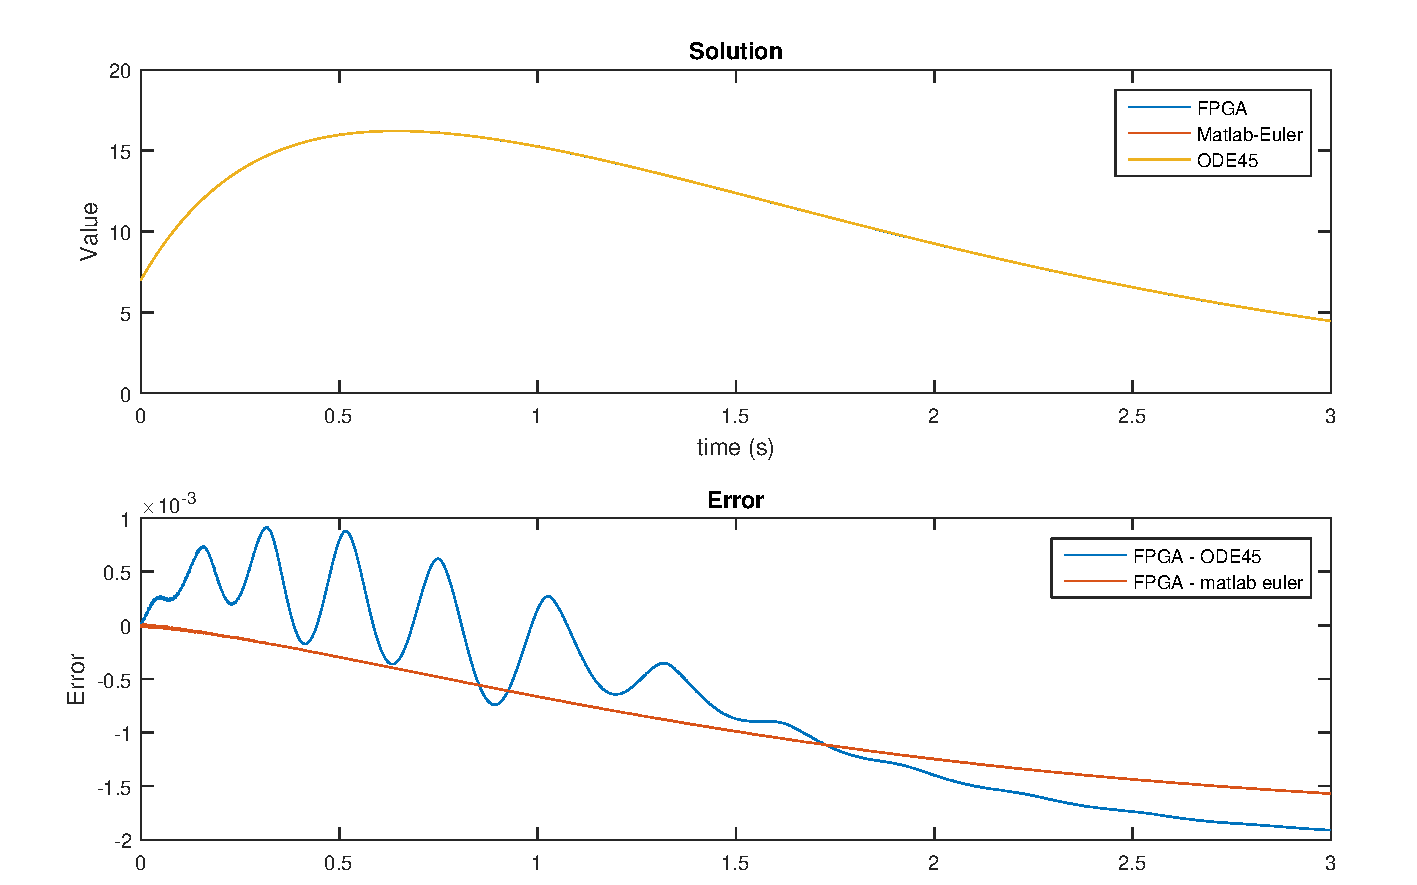
\includegraphics[width=0.9\textwidth]{euler_rv_ts=0,0001_os=10}
	\caption{Simplicity prevails: Euler's method attains better results than RK2 for all different time steps (h=1\e{-4}).}
	\label{f:euler_rv_ts=0,0001_os=10}
\end{figure}




